\maketitle

\section{任务分析}

由于 MacOS 以及 Windows 对于物理内存直接访问有着严格的限制,本实验在 Ubuntu 主机上完成,处于安全原因,由于 Linux 对物理地址直接访问文件\texttt{/dev/mem}的限制默认开启,只能查看前 1MB 的数据,见 \href{https://cateee.net/lkddb/web-lkddb/STRICT_DEVMEM.html}{Linux Kernel Driver DataBase},因此还需要修改内核实现。

\subsection{进程}

进程是操作系统中最基本的执行单元,是程序在其数据集上的一次执行过程。进程不仅包含程序代码,还包括程序计数器、寄存器、堆栈等信息。在现代操作系统中,进程是多任务的基础,通过调度系统可以让多个进程并行运行。

在本实验中,需要创建两个进程,且它们需要竞争进入临界区(Critical Section)。临界区是指多个进程共享的资源在同一时刻只能被一个进程访问的区域。

\subsection{临界区(Critical Section)}

临界区(Critical Section)是指一段程序代码,其中访问共享资源(如变量、文件、硬件等)时,多个进程或线程可能同时进入该区域,导致并发问题的发生。为了保证程序的正确性和数据的一致性,必须确保在同一时刻,只有一个进程或线程能够执行这段代码。否则,多个进程或线程可能会在没有适当同步的情况下对共享资源进行修改,从而引发竞态条件(race condition)和不可预期的结果。

在多进程或多线程环境下,操作系统需要采取措施来控制对临界区的访问,以防止出现这种竞态条件。通常,这些措施包括互斥锁、信号量、条件变量等同步机制。为了正确实现临界区的管理,操作系统需要提供一个机制来确保只有一个进程能够进入临界区,其他进程则必须等待,直到当前进程完成对共享资源的访问并退出临界区。

临界区问题的核心在于\textbf{互斥性}。互斥性意味着在任何时刻,只有一个进程或线程能够访问临界区。没有互斥,就可能导致共享资源的状态不一致,比如两个进程同时修改同一个变量,可能导致数据丢失或错误的计算结果。因此,在多任务操作系统中,解决临界区问题是保证程序正确执行的关键。

要解决临界区问题,需要引入进程或线程间的同步机制,这样在任意时刻,只有一个进程能够进入临界区,其他进程则需要等待。在早期的操作系统设计中,经典的 \textbf{Peterson 算法}就是一种为了解决两个进程的临界区竞争问题而提出的算法,它通过使用共享变量来控制两个进程的访问顺序,确保互斥。

临界区问题的解决不仅涉及互斥性,还可能涉及其他性质,例如死锁避免、进程的公平性(防止饥饿),以及进程或线程的并发执行效率。在实际应用中,操作系统使用多种方法来确保这些性质得到满足,确保系统的稳定和可靠运行。

\subsection{Peterson 算法}

Peterson 算法是一种经典的用于解决两个进程之间临界区竞争问题的算法,它通过使用两个共享变量来控制进程之间的进入和退出临界区的顺序,从而确保互斥性。这个算法由 Gary Peterson 在 1981 年提出,旨在为两个进程提供一个简单且有效的方式来解决竞争条件的问题,保证在任何时刻只有一个进程可以进入临界区,从而避免出现数据竞争。

Peterson 算法的核心思想是利用两个共享变量——\texttt{flag[2]} 和 \texttt{turn},来协调两个进程的执行顺序。\texttt{flag[i]} 用来表示进程 \texttt{i} 是否准备进入临界区,\texttt{turn} 则用来指示哪个进程应该进入临界区。具体地,\texttt{flag[i]} 是一个布尔变量,当进程 \texttt{i} 想要进入临界区时,它将 \texttt{flag[i]} 设置为 \texttt{true},表示它有意愿进入临界区。而 \texttt{turn} 是一个标记,表示当前应该由哪个进程进入临界区,进程 \texttt{i} 会将 \texttt{turn} 设置为另一个进程的编号,从而让对方优先进入临界区。

当进程准备进入临界区时,首先它会将自己的 \texttt{flag[i]} 设置为 \texttt{true},表示它想要进入临界区。然后,进程会将 \texttt{turn} 设置为另一个进程的编号,意图告诉对方如果它想要进入临界区,它应该先进入。接下来,进程会检查另一个进程的 \texttt{flag[j]},如果 \texttt{flag[j]} 为 \texttt{true},意味着另一个进程也准备进入临界区,那么它会查看 \texttt{turn} 是否指向自己。如果 \texttt{turn == j},表示轮到进程 \texttt{j} 进入临界区,那么进程 \texttt{i} 就会暂停,等待进程 \texttt{j} 执行完后再进入。只有当 \texttt{turn == i},或者 \texttt{flag[j] == false} 时,进程 \texttt{i} 才能进入临界区执行它的操作。

这种机制确保了互斥性,因为在任意时刻,只可能有一个进程进入临界区。当一个进程进入临界区并完成操作后,它会将自己的 \texttt{flag[i]} 设置为 \texttt{false},表示它退出临界区,其他进程就可以重新尝试进入。

Peterson 算法保证了多个重要的特性。首先是\textbf{互斥性},即在任何时刻只有一个进程能够进入临界区,从而避免了数据竞争的发生。其次是\textbf{无死锁性},即两个进程不会因为相互等待而导致死锁。再者,\textbf{有限等待}也得到保证,每个进程最终都会在有限的时间内进入临界区,不会被永久阻塞。此外,算法还保证了进程间的\textbf{公平性},即两个进程能够交替进入临界区,而不会导致某一个进程被长时间饿死。

尽管 Peterson 算法在理论上提供了一种有效的解决方案,但它在实际应用中受到一些限制。例如,它假设硬件提供原子性的读写操作,并且依赖于忙等待(busy waiting)机制,这在多处理器系统中可能导致性能问题。此外,随着进程数目的增加,Peterson 算法会变得不再适用,因为它仅适用于两个进程的情形,因此在更复杂的系统中,需要其他更加高效和通用的同步机制。

\subsection{逻辑地址与物理地址}

逻辑地址与物理地址的转换是本次实验的另一个重点。

逻辑地址和物理地址是计算机系统中与内存相关的两个重要概念,它们在操作系统和计算机体系结构中扮演着至关重要的角色。逻辑地址和物理地址之间的关系通过内存管理单元(MMU)来实现,是现代操作系统和硬件设计的基础。

逻辑地址,也叫做虚拟地址,是由程序在运行过程中生成的地址。当一个程序运行时,它并不知道它所使用的内存是如何在实际的物理内存中分配的,程序只是使用它所认为的“虚拟内存地址”。这些地址是程序在编译时或运行时生成的,通常是相对独立的,不直接与物理内存中的地址关联。操作系统和硬件会利用虚拟内存技术,通过一种叫做\textbf{地址映射}的机制,将这些虚拟地址转换成实际的物理地址。

物理地址是实际内存硬件中存储数据的地址,是计算机系统中内存的真实地址。物理内存指的是计算机中的实际内存芯片,它直接存储着所有的程序和数据。每个内存单元都有一个唯一的物理地址,CPU通过物理地址来访问这些内存单元。

在早期的计算机系统中,程序的逻辑地址和物理地址是相同的,也就是说,程序直接使用物理地址来访问内存。但是,随着操作系统和硬件的发展,尤其是在多任务操作系统和虚拟内存的引入后,程序使用的逻辑地址和实际的物理地址之间就产生了区分。这种区分使得操作系统可以在一个进程的虚拟地址空间和另一个进程的虚拟地址空间之间进行隔离,提高了系统的安全性和效率。

逻辑地址到物理地址的转换是通过内存管理单元(MMU)来完成的。MMU是计算机系统中的一个硬件部件,它负责将程序生成的虚拟地址转换成物理地址。转换的过程通常通过页表(Page Table)来实现。操作系统将虚拟内存划分为若干个\textbf{页}(Page),而物理内存则划分为若干个\textbf{帧}(Frame)。页表记录了虚拟页和物理帧之间的映射关系。当程序访问某个虚拟地址时,MMU会通过页表找到对应的物理地址,从而实现对实际内存的访问。

这种虚拟地址到物理地址的映射不仅提供了地址空间的隔离,防止了进程间直接访问彼此的内存,保护了系统的稳定性和安全性;同时,它也提供了内存的抽象和灵活性,使得操作系统可以更高效地管理内存。例如,操作系统可以将物理内存的不同部分分配给不同的进程,同时允许不同的进程在虚拟内存空间中拥有各自独立的地址空间,从而使得每个进程的地址空间看起来像是连续的、独立的,这种虚拟内存的概念极大地提高了系统的内存使用效率。

虚拟地址与物理地址的映射并不是一成不变的。操作系统,例如 Linux,可以通过一些技术,如\textbf{地址空间布局随机化}(ASLR)来随机化虚拟地址空间的布局,从而提高系统的安全性。页面置换算法也是一种操作系统管理虚拟内存的重要方式,它决定了哪些页面应该被保留在内存中,哪些页面应该被写回磁盘,从而优化内存的使用。

\section{实验环境}

\begin{itemize}
    \item 操作系统:ubuntu \texttt{20.04 LTS (Focal Fossa)}
    \item 内核版本:Linux kernel \texttt{5.15}
    \item 编程语言:c++23
    \item 编译器:GCC \texttt{14.2}
    \item 构建工具:xmake \texttt{v2.9.7+20241219}
    \item 文档构建工具:doxygen \texttt{1.12.0}
\end{itemize}

\section{设计思路}

\subsection{共享内存的创建和初始化}

为了让两个进程能够访问同一内存区域,我们使用了共享内存。共享内存是进程间通信(IPC)的一种方式,它允许多个进程访问同一块内存区域。在 Linux 系统中,可以使用 \texttt{mmap} 来创建和映射共享内存。通过使用 \texttt{MAP\_ANONYMOUS | MAP\_SHARED} 标志来创建匿名共享内存,这意味着内存区域没有与文件关联,并且共享给所有进程。

初始化时,我们将共享内存中的 \texttt{turn} 和 \texttt{flag} 变量设置为初始值,\texttt{turn} 设置为 0(表示进程 0 首先进入临界区),而 \texttt{flag} 数组初始化为 \texttt{false}(表示两进程都不想进入临界区)。

\subsection{Peterson 算法的实现}

Peterson 算法通过两个进程共享的变量 \texttt{turn} 和 \texttt{flag[]} 来协调进程对临界区的访问。每个进程在进入临界区之前,都将自己的 \texttt{flag[i]} 设置为 \texttt{true},并将 \texttt{turn} 设置为另一个进程的编号,表示自己愿意让对方先进入临界区。然后,进程检查另一个进程的 \texttt{flag[j]} 和 \texttt{turn},确保在对方希望进入时,它会等待。只有当对方不希望进入,或者轮到自己时,进程才能进入临界区。进入临界区后,进程会执行自己的任务,并在退出时将 \texttt{flag[i]} 设置为 \texttt{false},表示它已经完成并不再需要访问临界区。

该代码中通过 \texttt{peterson\_algorithm} 函数实现了每个进程的行为,其中包括请求进入临界区、执行临界区操作、退出临界区等步骤。该函数会循环执行 2 次,模拟进程反复请求进入临界区的情况。

伪代码如~\autoref{alg:peterson} 所示。

\begin{algorithm}[htbp]
\caption{Peterson Algorithm for Mutual Exclusion (for two processes)}
\label{alg:peterson}
\KwIn{Two processes with shared variables $flag[0], flag[1]$ and $turn$}
\KwOut{Mutual exclusion for both processes}
\SetKwFunction{FMain}{Peterson}
\SetKwProg{Fn}{Function}{:}{}
\Fn{\FMain{$i, j$}}{
    \While{True}{
        $flag[i] \gets True$ \tcp*{Process $i$ wants to enter critical section}
        $turn \gets j$ \tcp*{Give priority to process $j$}
        \While{$flag[j] \land turn = j$}{
            \tcp*{Busy waiting, process $i$ waits until process $j$ exits}
        }
        \tcp*{Critical section begins}
        \texttt{Enter critical section of process $i$}\;
        \texttt{Perform operations}\;
        \texttt{Exit critical section of process $i$}\;
        $flag[i] \gets False$ \tcp*{Process $i$ exits critical section}
    }
}
\end{algorithm}

\subsection{获取虚拟地址和物理地址}
虚拟内存(Virtual Memory)机制将一个进程的地址空间分为若干页(Page),通常每页大小为 4KB(用 \texttt{\_SC\_PAGESIZE} 获取)。操作系统通过页表维护虚拟地址到物理地址的映射关系。

\subsection{虚拟地址结构}
虚拟地址可以分解为两部分:
\begin{itemize}
    \item \textbf{页面号(Page Number)}:确定该虚拟地址属于哪一页。
    \item \textbf{页内偏移量(Offset)}:表示地址在页内的具体位置。
\end{itemize}

设页面大小为 $ Page Size$,则:
\begin{itemize}
    \item 高位 $Virtual Address / Page Size$ 表示页面号。
    \item 低位 $Virtual Address / Page Size$ 表示页内偏移量。
\end{itemize}

页表存储了虚拟页面与物理页帧的映射关系:
\begin{itemize}
    \item 每个虚拟页面对应一个条目,记录物理页帧号(Page Frame Number, PFN)。
    \item 页表条目中包含的其他标志位(例如有效位、读写权限位等)用于控制访问权限。
\end{itemize}

当 CPU 访问虚拟地址时,内存管理单元(MMU)会通过以下步骤进行地址转换:
\begin{itemize}
    \item 提取虚拟地址的页面号,查找页表中对应的物理页帧号。
    \item 将页帧号与页内偏移量组合,得到物理地址。
\end{itemize}

\texttt{/proc/self/pagemap} 是 Linux 中一个特殊的设备文件,详细解释可以看\href{https://www.kernel.org/doc/Documentation/vm/pagemap.txt}{Linux 官方文档},文件为用户态提供了当前进程虚拟地址到物理地址的映射信息。它是一个连续的二进制文件,按每页对应一个 64 位条目排列:
\begin{itemize}
    \item 第 63 位:页面是否驻留在物理内存中(Page Present)。
    \item 第 0 至 54 位:物理页帧号(PFN)。
\end{itemize}

文件索引与虚拟页号直接对应,因此可以通过计算虚拟地址的页号找到相关信息。

映射过程可以分为以下几步:
\begin{enumerate}
    \item \textbf{计算虚拟页号}
    \[
    \text{Page Number} = \text{Virtual Address} / \text{Page Size}
    \]
    \item \textbf{定位页表条目} \\
    每个页表条目占用 64 位(8 字节),因此可以通过偏移计算找到虚拟页号对应的条目位置:
    \[
    \text{Offset} = \text{Page Number} \times 8
    \]
    \item \textbf{读取条目信息} \\
    打开 \texttt{/proc/self/pagemap} 文件并跳转到计算出的偏移位置,读取 64 位数据。
    \item \textbf{解析条目信息} \\
    解析数据中的位信息:
    \begin{itemize}
        \item 第 63 位为页面存在标志。
        \item 第 0 至 54 位为物理页帧号。
    \end{itemize}
    \item \textbf{计算物理地址} \\
    然后便可以通过计算得到物理地址:
    \[
    \text{Physical Address} = (\text{PFN} \times \text{Page Size}) + (\text{Virtual Address} \& (\text{Page Size} - 1))
    \]
    其中:
    \begin{itemize}
        \item PFN:物理页帧号。
        \item $\text{Virtual Address} \& (\text{Page Size} - 1)$:页内偏移量。
    \end{itemize}
\end{enumerate}

转化成伪代码如~\autoref{alg:physical_address} 所示。

\begin{algorithm}[htbp]
    \caption{Get Physical Address and Verify}
    \label{alg:physical_address}
    \KwIn{Virtual address $vaddr$}
    \KwOut{Physical address $paddr$}
    
    \SetKwFunction{FMain}{virtual\_to\_physical\_address}
    \SetKwProg{Fn}{Function}{:}{}
    \Fn{\FMain{$vaddr$}}{
        $pagemap\_file \gets "/proc/self/pagemap"$\;
        $fd \gets open(pagemap\_file, O\_RDONLY | O\_CLOEXEC)$\;
        \If{$fd < 0$}{
            \Return{Failure, "Unable to open pagemap file"}
        }
        $page\_size \gets sysconf(\_SC\_PAGE\_SIZE)$\;
        $page\_number \gets \frac{vaddr}{page\_size}$\;
        $offset \gets vaddr \mod page\_size$\;
        
        $file\_offset \gets page\_number \times 8$\;
        $pagemap\_entry \gets read(fd, file\_offset)$\;
        
        \If{$pagemap\_entry \& (1 << 63) = 0$}{
            \Return{Failure, "Page not present"}
        }
        
        $pfn \gets pagemap\_entry \& ((1 << 54) - 1)$\;
        $physical\_addr \gets (pfn \times page\_size) + offset$\;
        
        \Return{physical\_addr}
    }
    \end{algorithm}

\subsection{物理地址验证}

在获得物理地址后,代码通过 \texttt{verify\_physical\_address} 函数来验证该物理地址是否正确。验证过程通过 \texttt{mmap} 和 \texttt{/dev/mem} 文件实现,详细文档见 \href{https://man7.org/linux/man-pages/man4/mem.4.html}{\texttt{dev/mem}} 与 \href{https://man7.org/linux/man-pages/man2/mmap.2.html}{\texttt{mmap}}。\texttt{/dev/mem} 也是 Linux 中一个特殊的设备文件,允许访问物理内存,正因如此,他的需求权限更高,并且默认屏蔽,前面提到的 \texttt{/proc/self/pagemap} 只需要 root 权限即可,该文件需要修改内核开启,否则只能访问前 1MB 的数据。通过在物理地址处读取数据,我们可以确认该物理地址是否正确。
\begin{itemize}
    \item 通过 \texttt{/dev/mem} 文件映射物理内存,读取物理地址对应位置的数据。
    \item 比较读取的值与期望值是否一致,从而验证物理地址的正确性。
\end{itemize}

\subsection{进程间同步和协作}

在主进程和子进程间通过共享内存传递数据,确保两进程能在相同的内存区域进行同步。在主进程中,首先通过 \texttt{fork()} 创建子进程,然后主进程和子进程各自执行 \texttt{peterson\_algorithm} 函数,模拟并发访问临界区。

两进程在访问临界区时,通过 Peterson 算法进行同步,确保在任一时刻,只有一个进程能够进入临界区执行操作。为了避免 CPU 占用过高,进程在等待时使用了 \texttt{sleep(100)},具体实现时,采用了线程安全的休眠方式,给 CPU 释放一定的时间,以减少不必要的忙等待。

\section{实现方法:修改 Linux 内核}
由于在现代 Linux 系统(如 Ubuntu)中,出于安全性和系统稳定性的考虑,对 \texttt{/dev/mem} 的访问受到严格限制。如果需要允许用户空间程序直接访问 \texttt{/dev/mem},需要通过重新配置并编译 Linux 内核来实现。考虑到没有给出实验说明,下面将详细给出操作过程,均为本人查看相关文档原创而来,建议老师可以考虑增加说明文档。

\subsection{获取内核源代码}

首先,需要获取 Linux 内核的源代码,以便进行更改。为了确保不引入其他问题,我们在对应的版本代码上进行修改,首先使用\texttt{uname} 命令查看自己的内核版本,我们的内核版本为 5.15:
\begin{bashcode}
  uname -r
\end{bashcode}
\begin{figure}[htbp]
    \centering
    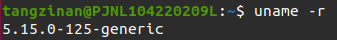
\includegraphics[width=0.5\textwidth]{images/uname.png}
    \caption{\texttt{uname} 命令查看内核版本}
\end{figure}

由于官方网站仅提供部分内核下载,且下载速度较慢,在\href{https://mirrors.edge.kernel.org/pub/linux/kernel/}{镜像网站}上找到对应的版本下载。
\begin{figure}[htbp]
    \centering
    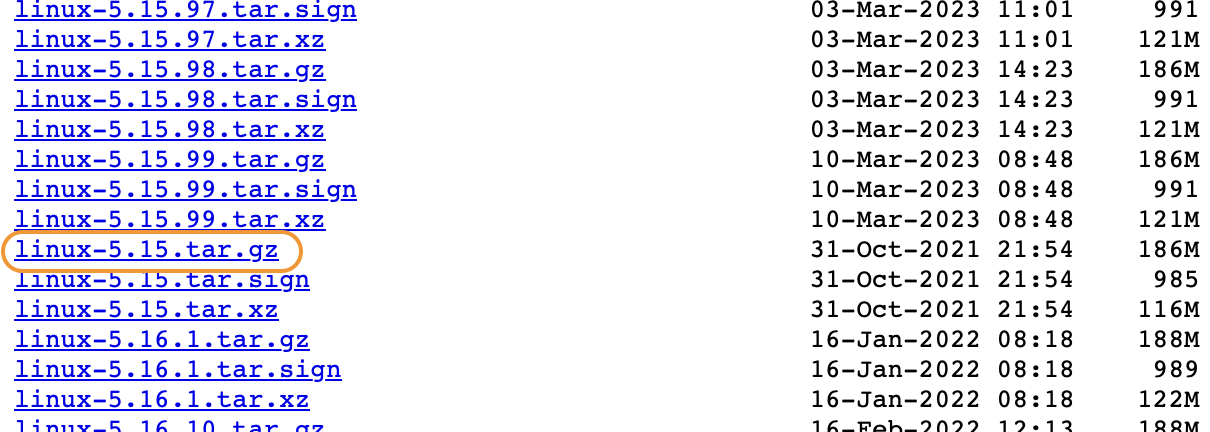
\includegraphics[width=0.5\textwidth]{images/download.png}
    \caption{从镜像网站下载 Linux 内核源代码}
\end{figure}
下载后的文件放入 \texttt{/usr/src/} 目录下。
\begin{bashcode}
    sudo mv linux-5.15.tar.gz /usr/src/ # 注意替换自己的版本号
\end{bashcode}

解压并进入通过包管理器下载的内核源代码:\begin{bashcode}
    cd /usr/src/
    sudo tar -xf linux-5.15.tar.gz # 注意替换自己的版本号
    cd linux-5.15 # 注意替换自己的版本号
\end{bashcode}

随后确保已安装编译内核所需的依赖包:
\begin{bashcode}
    sudo apt update
    sudo apt upgrade
    sudo apt-get install build-essential libncurses-dev bison flex libssl-dev libelf-dev dwarves zstd
\end{bashcode}

这些软件包包括编译工具链和库文件,用于配置和编译内核。

\subsection{配置内核}

首先需要复制系统当前的配置文件,否则新的内核可能不会启用当前系统中使用的某些硬件或驱动程序,如果某些功能或驱动程序没有被启用,可能会导致系统无法正常启动或部分硬件无法工作。
\begin{bashcode}
    cp /boot/config-$(uname -r) .config
\end{bashcode}

使用 \texttt{make menuconfig} 进行可视化配置,\texttt{menuconfig} 是一个基于文本的配置工具,可以通过图形界面选择和配置内核选项。
\begin{bashcode}
    sudo make menuconfig
\end{bashcode}

下面便是关键的内核修改配置。

为了便于区分自己修改的内核,首先选中 \texttt{General setup} $\to$ \texttt{Local version} 回车,设置自定义内核版本后缀,如 \texttt{-devmem}。
\begin{figure}[htbp]
    \centering
    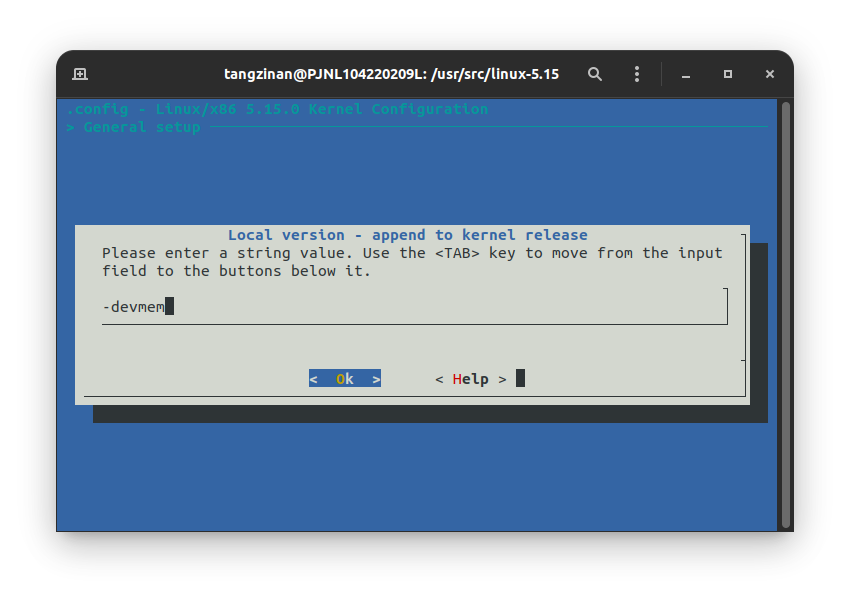
\includegraphics[width=0.6\textwidth]{images/devmem.png}
    \caption{设置自定义内核版本后缀}
\end{figure}

选中 \texttt{Kernel hacking} $\to$ \texttt{Filter access to /dev/mem} 选项,空格取消选择,以禁用 \texttt{CONFIG\_STRICT\_DEVMEM} 选项。这是一项安全功能,限制了用户空间程序对 \texttt{/dev/mem} 的访问,使得用户空间只能访问 1MB 的物理内存。由于不同版本的内核配置选项可能有所不同,具体选项可能会有所不同,但一般都会有类似的选项来控制对 \texttt{/dev/mem} 的访问。可以通过搜索关键字来查找选项,输入 \texttt{/} 后输入关键字进行搜索,可以看到对应的路径。修改后选择 \texttt{Save} 保存配置至 \texttt{.config} 文件。
\begin{figure}[htbp]
    \centering
    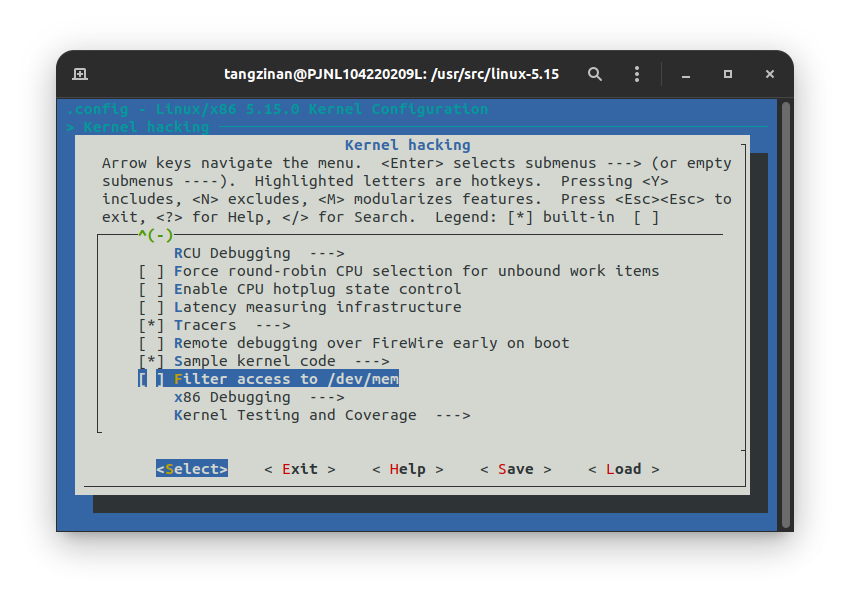
\includegraphics[width=0.6\textwidth]{images/filter.png}
    \caption{取消选项}
\end{figure}

此外,在较新的版本中,\texttt{HARDENED\_USERCOPY} 和 \texttt{HAVE\_HARDENED\_USERCOPY\_ALLOCATOR} 选项会导致 \texttt{CONFIG\_STRICT\_DEVMEM} 开启,路径为 \texttt{Security options} $\to$ \texttt{Harden memory copies between kernel and userspace},也需要确认这两个选项禁用(另外一个一般是默认禁用,可以用下面查看文件的方法检查)。

如果在 \texttt{menuconfig} 中找不到这些选项,可以直接编辑 \texttt{.config} 文件,将 \texttt{CONFIG\_STRICT\_DEVMEM} 设置为 \texttt{n},并将 \texttt{CONFIG\_HARDENED\_USERCOPY} 和 \texttt{CONFIG\_HAVE\_HARDENED\_USERCOPY\_ALLOCATOR} 设置为 \texttt{n},或者干脆将这些选项注释掉。

可以使用 \texttt{vim} 或者 \texttt{nvim} 进行修改,推荐使用 \texttt{nvim} 更新也更快,如果没有下载,使用 \texttt{sudo apt install} 下载,输入 \texttt{/} 即可进行查找。\texttt{vim} 的相关操作可见\href{https://github.com/wsdjeg/vim-galore-zh_cn}{Vim 从入门到精通}。
\begin{figure}[htbp]
    \centering
    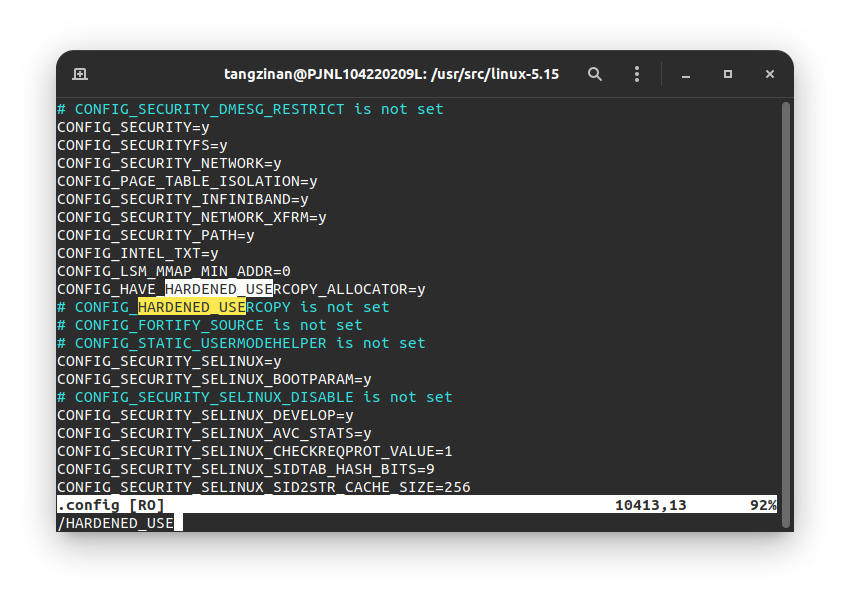
\includegraphics[width=0.6\textwidth]{images/vim.png}
    \caption{直接编辑配置文件}
\end{figure}

修改完配置后,还需要设置关闭启用模块签名,以便进行编译。
\begin{bashcode}
    scripts/config --disable SYSTEM_TRUSTED_KEYS
    scripts/config --disable SYSTEM_REVOCATION_KEYS
\end{bashcode}
因为我们自己修改的内核是没有经过签名的,那么在启用了 \texttt{SYSTEM\_TRUSTED\_KEYS} 和 \texttt{SYSTEM\_REVOCATION\_KEYS} 的情况下,内核会拒绝加载它们。禁用这些选项可以避免签名检查,允许加载没有签名的模块。

\subsection{编译和安装自定义内核}

首先清理之前的编译结果,避免对后续编译产生影响。
\begin{bashcode}
    sudo make clean
\end{bashcode}

使用以下命令并行编译(\texttt{-j\$(nproc)} 会根据的 CPU 核心数并行编译,加快编译速度):
\begin{bashcode}
    sudo make -j$(nproc)
\end{bashcode}

编译模块:
\begin{bashcode}
    sudo make modules
\end{bashcode}

编译内核映像:
\begin{bashcode}
    sudo make bzImage
\end{bashcode}

编译完成后,需要安装内核映像和模块到系统中。
\begin{bashcode}
    sudo make modules_install
\end{bashcode}
这将把编译好的模块安装到 \texttt{/lib/modules/<kernel-version>/} 目录下。

安装内核映像。
\begin{bashcode}
    sudo make install
\end{bashcode}
此命令会将内核映像(如 \texttt{vmlinuz-<version>})、系统映像和内核配置文件安装到 \texttt{/boot/} 目录,并自动更新引导加载器(如 GRUB)。

\subsection{重启并更换内核}

为了防止不显示 GRUB 菜单,我们先修改 GRUB 配置。
\begin{bashcode}
    sudo nvim /etc/default/grub
\end{bashcode}
将 \texttt{GRUB\_TIMEOUT} 设置为一个较大的值,如 10 秒,以确保 GRUB 菜单显示,并注释掉 \texttt{GRUB\_HIDDEN\_TIMEOUT}。
\begin{figure}[htbp]
    \centering
    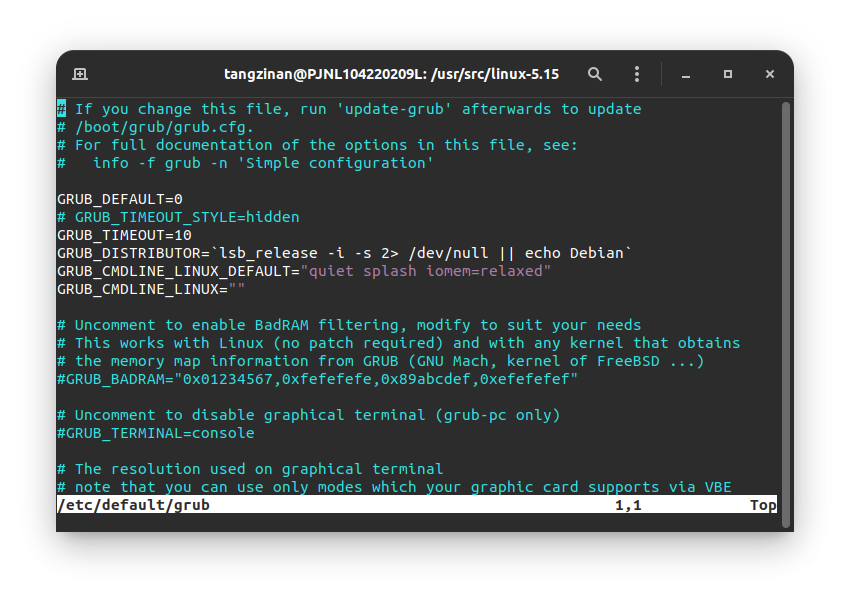
\includegraphics[width=0.6\textwidth]{images/grup.png}
    \caption{编辑 GRUP 配置文件}
\end{figure}

手动更新 GRUB 配置:
\begin{bashcode}
    sudo update-grub
\end{bashcode}

随后重启系统:
\begin{bashcode}
    sudo reboot
\end{bashcode}

在启动时按住 Shift 键(对于 BIOS 系统,常见于虚拟机)或 Esc 键(对于 UEFI 系统)以显示菜单。在系统启动时,GRUB 菜单将显示多个内核选项。选择 \texttt{Advanced options for Ubuntu},然后选择新安装(此前我们已经设置过后缀)的内核版本,启动系统。

\subsection{验证内核配置}

有时候会因为 Nvidia 掉驱动导致无法正常启动页面,在 \texttt{Advanced options for Ubuntu} 菜单中选择对应 \texttt{recovery mode},首先选择 \texttt{network} 连接网络,再选择 \texttt{dpkg} 修复包即可。

进入系统后,再次 \texttt{uname -r} 查看内核版本,确保已经切换到新内核。
\begin{figure}[htbp]
    \centering
    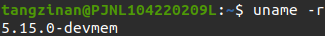
\includegraphics[width=0.6\textwidth]{images/change.jpeg.png}
    \caption{已经切换到新内核}
\end{figure}

\section{系统框架及关键代码}

\subsection{\texttt{main()} 函数}

\texttt{main()} 函数是程序的入口。

\subsubsection{分配共享内存}
查看文档,\texttt{mmap} 函数可以被用来创建共享内存,其借口定义如下:\begin{cppcode}
void *mmap(void *addr, size_t length, int prot, int flags, int fd, off_t offset);
\end{cppcode} 
\begin{enumerate}
    \item \texttt{void *addr}
    \begin{itemize}
        \item \textbf{含义}:建议的映射起始地址。
        \item \textbf{作用}:
        \begin{itemize}
            \item 如果为 \texttt{NULL},则表示让内核自动选择映射地址。
            \item 如果不为 \texttt{NULL},内核会尝试将映射放在指定地址(可能会失败)。
        \end{itemize}
        \item \textbf{注意}:
        \begin{itemize}
            \item 通常设置为 \texttt{NULL} 以让内核选择最合适的地址。
        \end{itemize}
    \end{itemize}

    \item \texttt{size\_t length}
    \begin{itemize}
        \item \textbf{含义}:映射的内存区域大小(以字节为单位)。
        \item \textbf{作用}:
        \begin{itemize}
            \item 指定映射区域的长度。
            \item 映射的区域会从 \texttt{offset} 开始,向后延续 \texttt{length} 字节。
        \end{itemize}
        \item \textbf{注意}:
        \begin{itemize}
            \item 必须为系统页大小(通常是 4KB)的倍数,否则会向上对齐到页大小。
        \end{itemize}
    \end{itemize}

    \item \texttt{int prot}
    \begin{itemize}
        \item \textbf{含义}:内存保护属性。
        \item \textbf{取值}:可以是以下宏的组合(通过按位或 \texttt{|} 连接):
        \begin{itemize}
            \item \texttt{PROT\_READ}:可读。
            \item \texttt{PROT\_WRITE}:可写。
            \item \texttt{PROT\_EXEC}:可执行。
            \item \texttt{PROT\_NONE}:不可访问。
        \end{itemize}
        \item \textbf{示例}:
        \begin{itemize}
            \item 只读:\texttt{PROT\_READ}
            \item 可读写:\texttt{PROT\_READ | PROT\_WRITE}
        \end{itemize}
    \end{itemize}

    \item \texttt{int flags}
    \begin{itemize}
        \item \textbf{含义}:映射类型和属性标志。
        \item \textbf{取值}:以下标志可以单独使用或组合:
        \begin{itemize}
            \item 映射类型(必选之一):
            \begin{itemize}
                \item \texttt{MAP\_SHARED}:共享映射。对内存区域的修改会写回到文件,并对其他进程可见。
                \item \texttt{MAP\_PRIVATE}:私有映射。对内存区域的修改不会影响原文件或其他进程。
            \end{itemize}
            \item 其他标志(可选):
            \begin{itemize}
                \item \texttt{MAP\_ANONYMOUS}:匿名映射,不与文件关联(\texttt{fd} 必须为 \texttt{-1})。
                \item \texttt{MAP\_FIXED}:强制使用 \texttt{addr} 指定的地址。如果地址不可用,会失败。
                \item \texttt{MAP\_POPULATE}:预先加载页表。
            \end{itemize}
        \end{itemize}
    \end{itemize}

    \item \texttt{int fd}
    \begin{itemize}
        \item \textbf{含义}:要映射的文件描述符。
        \item \textbf{作用}:
        \begin{itemize}
            \item 指定需要映射的文件。
            \item 如果使用匿名映射(\texttt{MAP\_ANONYMOUS}),必须设置为 \texttt{-1}。
        \end{itemize}
        \item \textbf{注意}:
        \begin{itemize}
            \item 文件描述符必须支持读取或读写(根据 \texttt{prot})。
        \end{itemize}
    \end{itemize}

    \item \texttt{off\_t offset}
    \begin{itemize}
        \item \textbf{含义}:映射区域在文件中的偏移量。
        \item \textbf{作用}:
        \begin{itemize}
            \item 指定映射的起始位置,必须是系统页大小(通常是 4KB)的倍数。
        \end{itemize}
        \item \textbf{注意}:
        \begin{itemize}
            \item 如果不是页大小的倍数,映射会失败。
        \end{itemize}
    \end{itemize}
\end{enumerate}

返回值:\begin{itemize}
    \item 成功:返回指向映射区域的指针。
    \item 失败:返回 \texttt{MAP\_FAILED}(即 \texttt{(void *)-1}),并设置 \texttt{errno}。
\end{itemize}

\begin{cppcode}
int* shared_mem = static_cast<int*>(mmap(nullptr, sizeof(int) * 3, PROT_READ | PROT_WRITE, MAP_SHARED | MAP_ANONYMOUS, -1, 0));
\end{cppcode}

使用 \texttt{mmap} 创建了一个匿名共享内存区域,用于在父子进程间共享数据。分配了3个 \texttt{int} 大小的区域,用于存放 \texttt{flag} 和 \texttt{turn}。

\subsubsection{初始化共享变量}
\begin{cppcode}
volatile int* flag = reinterpret_cast<volatile int*>(shared_mem);
volatile int* turn = reinterpret_cast<volatile int*>(shared_mem + 2);
flag[0] = 0;
flag[1] = 0;
*turn = 0;
\end{cppcode}
初始化两个进程的 \texttt{flag} 值为0,表示开始时均无意进入临界区,\texttt{turn} 设置为0表示在冲突时优先让进程0先尝试进入。在多线程或多进程共享内存中如果使用普通 \texttt{int} 可能被编译器或 CPU 缓存重排,从而破坏算法预期。因此使用 \texttt{volatile} 限定符,强制编译器不优化相关内存访问。

\subsubsection{创建子进程}
\begin{cppcode}
pid_t pid = fork();
\end{cppcode}
使用 \texttt{fork()} 创建子进程,形成两个进程,父进程 \texttt{pid>0},使用 \texttt{i=0},子进程 \texttt{pid=0},使用 \texttt{i=1}。父进程在完成自身的临界区访问后使用 \texttt{wait(nullptr)} 等待子进程结束,然后使用 \texttt{munmap} 解除内存映射,释放资源。

\subsection{Peterson 算法:\texttt{peterson\_algorithm()} 函数}
\begin{cppcode}
for (int count = 0; count < 2; count++) {
    flag[i] = 1;    // 表示进程 i 想进入临界区
    *turn = j;      // 将 turn 设为对方,这意味着若两者同时想进,则优先让对方进

    // 忙等待 (busy-wait)
    while ((flag[j] != 0) && (*turn == j)) {
        // 当对方想进入临界区且 turn 指向对方时,当前进程等待
    }

    // ---- 临界区开始 ----
    std::cout << "Process " << i << " entered critical section (iteration " << count << ")\n";

    // 验证共享变量 turn 的物理地址及值的一致性
    verify_physical_address(turn, i);

    // 模拟在临界区工作的时间
    std::this_thread::sleep_for(std::chrono::seconds(1));
    std::cout << "Process " << i << " leaving critical section (iteration " << count << ")\n\n";

    // 离开临界区,释放权利
    flag[i] = 0;

    // 为了更好的演示效果,等待一段时间,让对方有机会进入临界区
    std::this_thread::sleep_for(std::chrono::seconds(1));
}
\end{cppcode}
实现方法与前文所述的伪代码一致,通过 \texttt{flag} 和 \texttt{turn} 变量实现进程间的同步。值得注意的是,由于需要验证物理地址正确,正好可以将临界区行为设置为验证物理地址。此外,我们没有使用普通的 \texttt{sleep()} 函数,而是使用了线程安全的 \texttt{std::this\_thread::sleep\_for()} 函数,该函数专为 C++ 线程设计,明确表示让当前线程暂停执行,语义更加清晰,以避免在多线程环境下可能出现的问题。

\subsection{获取物理地址:\texttt{virtual\_to\_physical\_address()} 函数}
实现将虚拟地址转换为物理地址的核心逻辑。

首先确定系统页面的大小
\begin{cppcode}
auto page_size = static_cast<uint64_t>(sysconf(_SC_PAGESIZE));
\end{cppcode}

根据虚拟地址与页面大小计算在 \texttt{pagemap} 文件中的偏移:
\begin{cppcode}
uint64_t offset = (vaddr / page_size) * sizeof(uint64_t);
\end{cppcode}

打开 pagemap 文件并定位:
\begin{cppcode}
FILE* pagemap = fopen("/proc/self/pagemap", "rbe");
fseek(pagemap, static_cast<int64_t>(offset), SEEK_SET);
\end{cppcode}

读取对应的 64 位条目 e:
\begin{cppcode}
fread(&e, sizeof(uint64_t), 1, pagemap);
\end{cppcode}
条目 \texttt{e} 中包含该虚拟页对应的物理页帧号(PFN)以及其他标志位。当 \texttt{e} 的最高位(第63位)为1时,表示此页已映射到物理内存。

提取 PFN 并计算物理地址:
\begin{cppcode}
uint64_t pfn = e & ((1ULL << 54U) - 1);
paddr = pfn * page_size + (vaddr & (page_size - 1));
\end{cppcode}
\texttt{pfn} 是物理页帧号,通过 \texttt{pfn * page\_size} 得到物理页的起始地址,然后加上 \texttt{vaddr} 在页面内的偏移量得到完整的物理地址。

值得注意的是,在实现时我们使用了 \texttt{static\_cast} 以及 \texttt{reinterpret\_cast} 等 C++ 强制类型转换,编译器可以严格检查转换是否合法。例如,它可以在编译期捕捉明显错误。这样做更现代化、符合类型安全且可读性更高,能够明确表达意图,并有效减少不安全的类型转换带来的隐患。为了保证跨平台一致性,使用 \texttt{uint64\_t} 而不是 \texttt{long} 来定义相关变量。

\subsection{验证物理函数正确:\texttt{verify\_physical\_address()} 函数}
通过验证共享内存中 \texttt{turn} 的物理地址对应的值与当前进程逻辑访问该地址的值是否一致,从而说明进程间通过共享内存访问同一物理地址。

首先获取 \texttt{turn} 的虚拟地址并转换为物理地址
\begin{bashcode}
auto vaddr = reinterpret_cast<uintptr_t>(turn);
uintptr_t paddr = virtual_to_physical_address(vaddr);
\end{bashcode}

若转换成功(\texttt{paddr != 0}),则打开 \texttt{/dev/mem},通过 \texttt{lseek} 定位到 \texttt{paddr} 对应的物理位置,然后 \texttt{read} 读取该处的内存值。
\begin{cppcode}
int memfd = open("/dev/mem", O_RDONLY | O_CLOEXEC);
// ...
ssize_t rd = read(memfd, &val_at_paddr, sizeof(val_at_paddr));
\end{cppcode}

将从物理地址读取到的 \texttt{val\_at\_paddr} 与逻辑读取的 \texttt{*turn} 值进行比较,并根据是否相等输出验证结果。

\section{模块流程图}

由 doxygen 自动生成。

\begin{figure}[H]
    \centering
    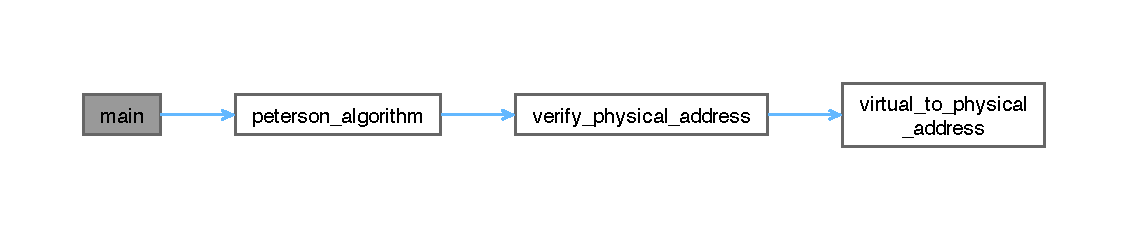
\includegraphics[width=0.7\textwidth]{images/flow.pdf}
    \caption{模块流程图}
\end{figure}

\section{测试}

在任一时刻只有一个进程进入临界区,此外,通过物理地址直接访问的 \texttt{turn} 值与预期值一致,说明了物理地址的正确性。

\begin{figure}[H]
    \centering
    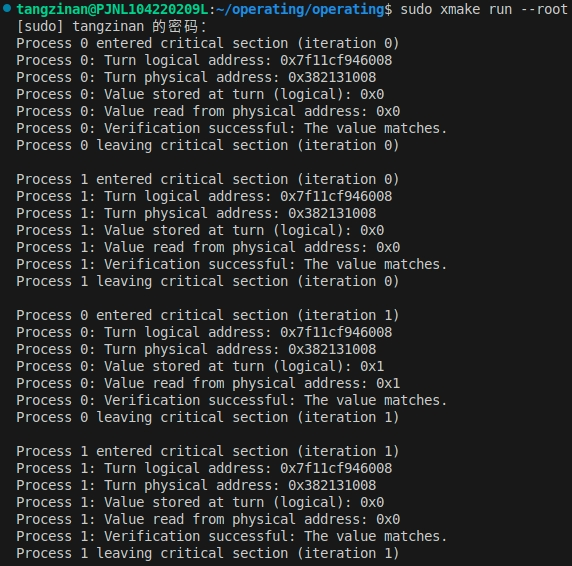
\includegraphics[width=0.7\textwidth]{images/res.jpeg}
    \caption{程序运行结果}
\end{figure}

\appendix

\section{程序文档 by doxygen}

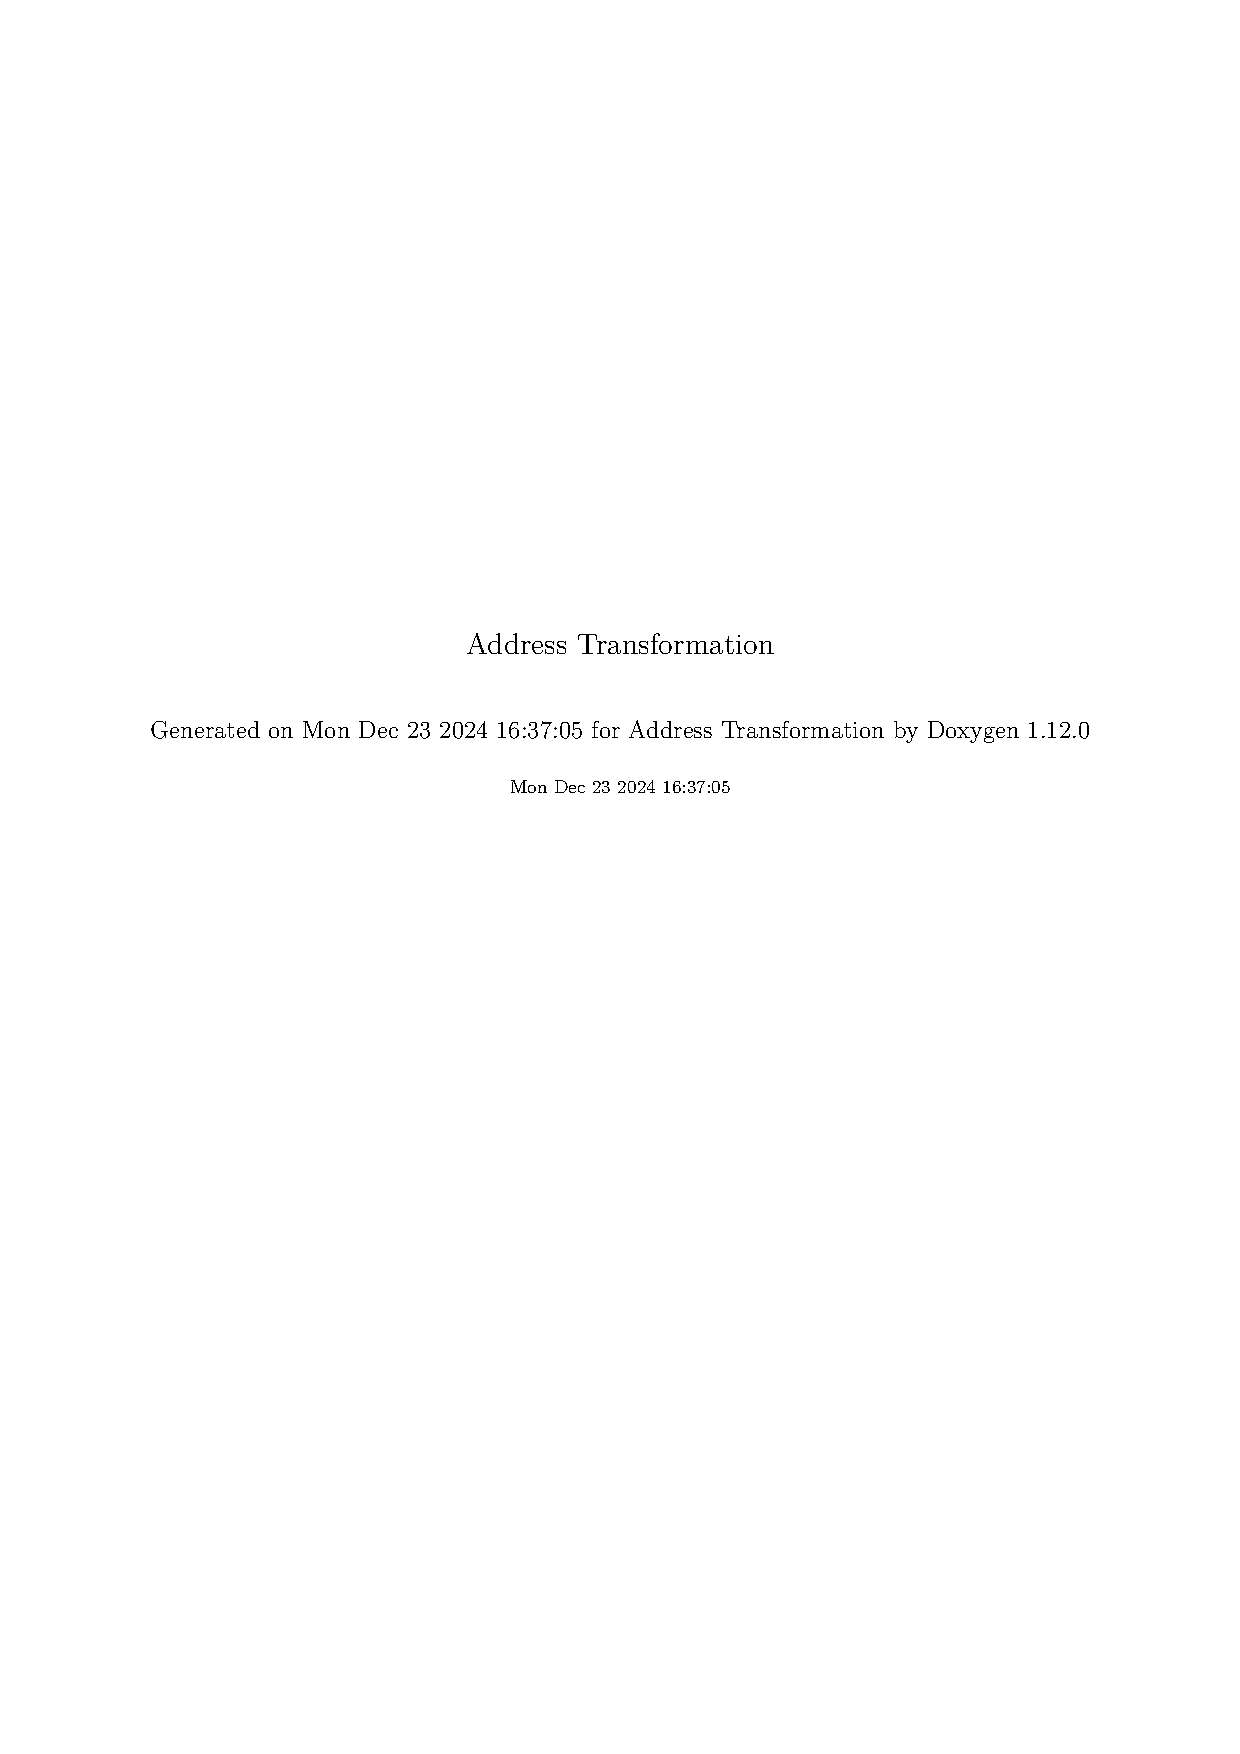
\includepdf[pages=-]{refman.pdf}